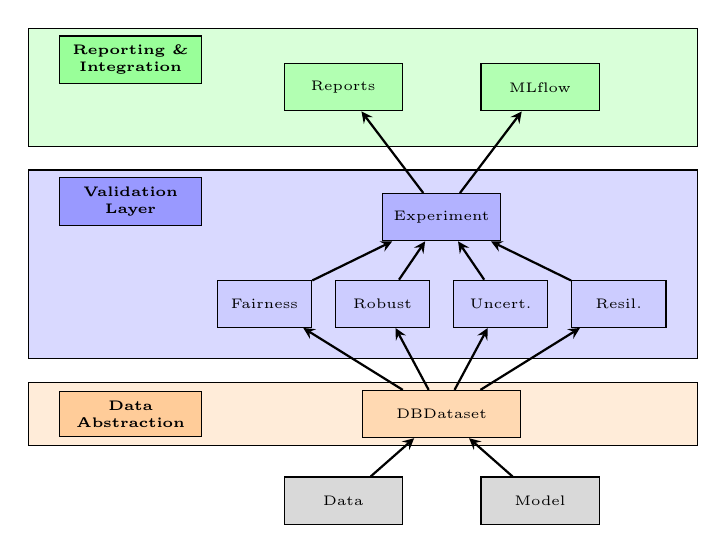
\begin{tikzpicture}[
    component/.style={rectangle, draw, minimum width=1.5cm, minimum height=0.6cm, align=center, font=\tiny},
    arrow/.style={->, >=stealth, thick}
]

% Background boxes - ajustados para não sobrepor
\draw[fill=green!15, draw] (-4.5,1.0) rectangle (4.0,-0.5);
\draw[fill=blue!15, draw] (-4.5,-0.8) rectangle (4.0,-3.2);
\draw[fill=orange!15, draw] (-4.5,-3.5) rectangle (4.0,-4.3);

% Layer labels - posicionados à esquerda, fora dos componentes
\node[rectangle, draw, fill=green!40, minimum width=1.8cm, minimum height=0.5cm, font=\tiny\bfseries, align=center] at (-3.2,0.6) {Reporting \&\\Integration};
\node[rectangle, draw, fill=blue!40, minimum width=1.8cm, minimum height=0.5cm, font=\tiny\bfseries, align=center] at (-3.2,-1.2) {Validation\\Layer};
\node[rectangle, draw, fill=orange!40, minimum width=1.8cm, minimum height=0.5cm, font=\tiny\bfseries, align=center] at (-3.2,-3.9) {Data\\Abstraction};

% Layer 3: Reporting - Components
\node[component, fill=green!30] (report) at (-0.5,0.25) {Reports};
\node[component, fill=green!30] (mlflow) at (2,0.25) {MLflow};

% Layer 2: Validation - Components
\node[component, fill=blue!30] (exp) at (0.75,-1.4) {Experiment};
\node[component, fill=blue!20, minimum width=1.2cm] (f1) at (-1.5,-2.5) {Fairness};
\node[component, fill=blue!20, minimum width=1.2cm] (f2) at (0,-2.5) {Robust};
\node[component, fill=blue!20, minimum width=1.2cm] (f3) at (1.5,-2.5) {Uncert.};
\node[component, fill=blue!20, minimum width=1.2cm] (f4) at (3,-2.5) {Resil.};

% Layer 1: Data - Components
\node[component, fill=orange!30, minimum width=2cm] (db) at (0.75,-3.9) {DBDataset};

% Input
\node[component, fill=gray!30] (data) at (-0.5,-5.0) {Data};
\node[component, fill=gray!30] (model) at (2,-5.0) {Model};

% Arrows
\draw[arrow] (data) -- (db);
\draw[arrow] (model) -- (db);
\draw[arrow] (db) -- (f1);
\draw[arrow] (db) -- (f2);
\draw[arrow] (db) -- (f3);
\draw[arrow] (db) -- (f4);
\draw[arrow] (f1) -- (exp);
\draw[arrow] (f2) -- (exp);
\draw[arrow] (f3) -- (exp);
\draw[arrow] (f4) -- (exp);
\draw[arrow] (exp) -- (report);
\draw[arrow] (exp) -- (mlflow);

\end{tikzpicture}